%%%%%%%%%%%%%%%%%%%%%%%%%%%%%%%%%%%%%%%%%%%%%%%%%%%%%%%%%%%%%%%%%%%%%%%%%%%%%%%%%%%%%%%%%%%%%
%%									Chapitre 1											%
%%%%%%%%%%%%%%%%%%%%%%%%%%%%%%%%%%%%%%%%%%%%%%%%%%%%%%%%%%%%%%%%%%%%%%%%%%%%%%%%%%%%%%%%%%%%%
\chapter{An Overview of the Thesis}\label{chap:intro}
	\citationChap{
	The thing about quotes on the internet is that you can not confirm their validity
	}{Abraham Lincoln}
	\minitoc
	\newpage

%%%%%%%%%%%%%%%%%%%%%%%%%%%%%%%%%%%%%%%%%%%%%%%%%%%%%%%%%%%%%%%%%%%%%%%%%%%%%%%%%%%%%%%%%%%%%



% Début du chapitre

\section{Context of the Thesis}\label{sec:intro.context}
	\subsection{What do we study and why?}\label{sec:intro.context.what}
	    
	\gls{mab}

% 	\begin{tableth}
% 		\caption[Légende courte pour l'exemple de tableau]{Un tableau avec une légende tellement longue que ce serait hideux dans la liste des tableaux}
% 			\label{tab:exemple}
% 		\begin{tabular}{c|c}
% 			Coucou	& Au revoir\\
% 			\hline
% 			maman	& papa
% 		\end{tabular}
% 	\end{tableth}

% 	\begin{figureth}
% 		\begin{subfigureth}{0.4\textwidth}
% 			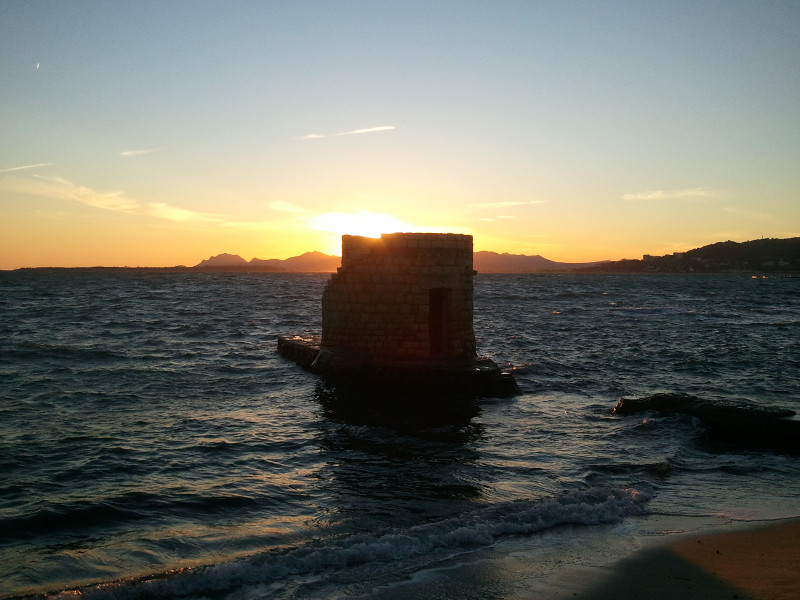
\includegraphics[width=\linewidth]{Chapter1/img/Antibes}
% 			\caption{Photo du Cap d'Antibes}
% 				\label{sub:Antibes}
% 		\end{subfigureth}
% 		\begin{subfigureth}{0.4\textwidth}
% 			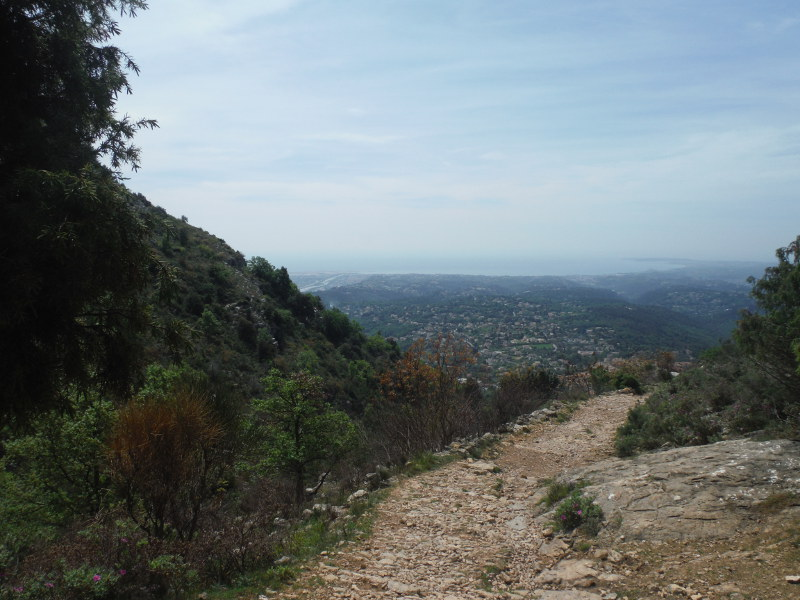
\includegraphics[width=\linewidth]{Chapter1/img/SaintJeannet}
% 			\caption{Saint Jeannet, depuis son Baou}
% 				\label{sub:SaintJeannet}
% 		\end{subfigureth}
% 		\caption[Légende courte pour la figure]{Exemple d'utilisation des sous-figures. J'utilise ici volontairement une légende longue.}
% 			\label{fig:exemple}
% 	\end{figureth}

\section{Multi-Armed Bandits and Optimization}\label{sec:intro.mab}
    
\section{A Summary of the Contributions}\label{sec:intro.contributions}

\paragraph{Included in this thesis}

\cite{shang2018adaptive,shang2019dttts,shang2019adaptive,shang2020dttts,degenne2020game,shang2020t3c}.

\paragraph{Not included in this thesis}

\cite{shang2020vector,shang2021safe,menard2021ucbmq}.

\cite{rlberry2021}.

\section{Organization of the Thesis}\label{sec:intro.organization}

% \newpage
% \bibliographystyle{plain}
% \bibliography{library}
